\documentclass{beamer}
\usepackage[utf8]{inputenc}
\usepackage{graphicx}

\newtheorem{definicion}{Definición}
\newtheorem{ejemplo}{Ejemplo}

%%%%%%%%%%%%%%%%%%%%%%%%%%%%%%%%%%%%%%%%%%%%%%%%%%%%%%%%%%%%%%%%%%%%%%%%%%%%%%%
\title[Búsqueda de raíces mediante el método de Newton - Raphson ]{Método Newton}
\author[Tecnicas Experimentales]{Alba Crespo Perez, Raquel Espino Mantas y Robbert Jozef Michiels}
\date[12-05-2014]{12 de mayo de 2014}
%%%%%%%%%%%%%%%%%%%%%%%%%%%%%%%%%%%%%%%%%%%%%%%%%%%%%%%%%%%%%%%%%%%%%%%%%%%%%%%

%\usetheme{Madrid}
%\usetheme{Antibes}
%\usetheme{tree}
%\usetheme{classic}

%%%%%%%%%%%%%%%%%%%%%%%%%%%%%%%%%%%%%%%%%%%%%%%%%%%%%%%%%%%%%%%%%%%%%%%%%%%%%%%
\begin{document}
  
%++++++++++++++++++++++++++++++++++++++++++++++++++++++++++++++++++++++++++++++
\begin{frame}
  \titlepage
  \begin{small}
    \begin{center}
     Facultad de Matemáticas \\
     Universidad de La Laguna
    \end{center}
  \end{small}

\end{frame}
%++++++++++++++++++++++++++++++++++++++++++++++++++++++++++++++++++++++++++++++

%++++++++++++++++++++++++++++++++++++++++++++++++++++++++++++++++++++++++++++++
\begin{frame}
  \frametitle{Índice}
  \tableofcontents[pausesections]
\end{frame}
%++++++++++++++++++++++++++++++++++++++++++++++++++++++++++++++++++++++++++++++


\section{Motivación y objetivos}


%++++++++++++++++++++++++++++++++++++++++++++++++++++++++++++++++++++++++++++++
\begin{frame}

\frametitle{Motivación y objetivos}

  
El objetivo principal del presente trabajo reside en la implementación, mediante
el uso del lenguaje de programación Python, de un algoritmo basado en el método
de Newton - Raphson que nos permita llevar a cabo el cálculo de las raíces de la
función $f(x) = cos(\pi x)$.

Además, se pretende lograr la consecución de los siguientes objetivos específicos:
  \begin{itemize}
  \item
  Efectuar un análisis numérico y gráfico de la evolución en el número de 
  iteraciones requeridas por este método para la obtención de una raíz, en
  función del error absoluto de la estimación inicial tomada como punto de 
  partida del método respecto a la solución real determinada tras su aplicación.
  \pause
  \item
   Analizar el costo computacional, en términos de tiempo de uso de CPU, asociado 
   a la ejecución del algoritmo implementado, así como su variabilidad y sensibilidad
   ante modificaciones en los parámetros iniciales.
  \end{itemize}

\end{frame}
%++++++++++++++++++++++++++++++++++++++++++++++++++++++++++++++++++++++++++++++

\section{Fundamentos teóricos}

%++++++++++++++++++++++++++++++++++++++++++++++++++++++++++++++++++++++++++++++
\begin{frame}

\frametitle{Breve introducción historica}


Este método constituye una vía algorítmica de análisis numérico destinada a la 
determinación de los ceros o raíces de una función matemática dada. Su primera 
descripción relevante fue desarrollada por el multidisciplinar científico inglés 
Isaac Newton en su obra \emph{De analysi per aequationes numero terminorum infinitas}, 
escrita en 1669 y publicada en 1711 por William Jones, así como en su tratado \emph{De 
metodis fluxionum et serierum infinitarum}, editado en 1736 por John Colson bajo el título 
de \emph{Método de las fluxiones}.

Sin embargo, si bien su reconocimiento no alcanzó en su momento la repercusión otorgada a
los trabajos de Newton, dicho método encuentra mención previa en el libro \emph {Aequationum 
Universalis} (1690), cuya publicación conllevó para su autor, el matemático inglés Joseph 
Raphson, la consecución del ingreso en la \emph{Royal Society} de Londres.  

\end{frame} 

\begin{frame}

\frametitle{Descripción teórica del método}


 
Para utilizar el método de Newton-Raphson es necesario comenzar con un valor inicial 
suficientemente cercano a la raíz buscada, que a medida que avance la ejecución del 
algoritmo progresará acercándose al valor real de esta raíz 

Una vez fijada una estimación inicial $x_{0}$ calcularemos la expresión de la recta 
tangente a la gráfica de la función dada en el punto $x = x_{0}$. La coordenada de 
corte de dicha recta con el eje horizontal será considerada de modo genérico como un
valor más cercano a la raíz buscada que la hipótesis original, por lo que este paso 
podrá aplicarse de forma recursiva tomando como suposición al nuevo valor obtenido, 
hasta lograr una aproximación aceptable de la raíz dentro de un margen de tolerancia 
fijado de antemano de acuerdo con la precisión exigida por el contexto.

\end{frame}

\begin{frame}

Profundizaremos ahora en los cálculos matemáticos necesarios para la obtención de una
expresión recursiva del algoritmo. Sabemos que la expresión de una recta de pendiente 
\emph{m} y que pasa por el punto $(a, b)$ viene dada de la forma:

$$ y - b = m (x - a)$$

En consecuencia, y considerando que la pendiente de la recta tangente a una función $f(x)$
en un punto $x = x_{0}$ corresponde al valor en dicho punto de su primera derivada, obtenemos 
la siguiente expresión para dicha recta en la denominada \emph{forma punto-pendiente}:

$$y - f(x_{0}) = f'(x_{0}) (x - x_{0})$$

\end{frame}

\begin{frame}

Tomando $y = 0$, procedemos a determinar el punto de corte de la recta anterior con el eje de
abscisas. La notación $x_{n+1}$ indica que el valor resultante de \emph{x} corresponderá a la
estimación tomada como partida para la siguiente ejecución del algoritmo:


$$y = 0 \ \ \to \ \ -f(x_{0}) = f'(x_{0}) (x_{n+1} - x_{0}) \ \ \to \ \ x_{0} f'(x_{0}) - f(x_{0}) 
= x_{n+1} f'(x_{0}) \ \ \to $$

$$\to \ \ x_{n+1} = x_{0} - \frac{f(x_{0})}{f'(x_{0})}$$

De acuerdo con lo comentado al inicio de la sección, observamos que las funciones con acentuadas
variaciones de pendiente en el entorno de la raíz buscada dificultarán la convergencia del algoritmo,
por lo que al llevar a cabo su implementación computacional será preciso establecer una cota máxima
de iteraciones con el fin de evitar que la ejecución recursiva permanezca atrapada en un patrón
de divergencia.

\end{frame}

%++++++++++++++++++++++++++++++++++++++++++++++++++++++++++++++++++++++++++++++++++++++++++++++++

\section{Análisis de la función de estudio}

%++++++++++++++++++++++++++++++++++++++++++++++++++++++++++++++++++++++++++++++++++++++++++++++++
\begin{frame}

\frametitle{Ánalisis de la función de estudio}
Con el objetivo de lograr una mejor comprensión de los resultados obtenidos en la aproximación de
las raíces de la función $f(x) = cos (\pi x)$ mediante el algoritmo de Newton-Raphson, procedemos 
a calcular dichas raíces de modo teórico, mediante la resolución de una sencilla ecuación trigonométrica:

$$cos (\pi x) = 0 \ \ \to \ \ \pi x = \frac{\pi}{2} + k \pi, k \in \mathbb{Z} \ \ \to x = \frac{1}{2} +
k, \ k \in \mathbb{Z}$$

Vemos así que se verifica lo siguiente:

$$cos (\pi x) = 0 \iff x = ..., -2.5, -1,5, -0.5, 0.5, 1.5, 2.5, ...$$


\end{frame}

\begin{frame}

Concluimos con ello que se trata de una función periódica con periodo P = 2. Este hecho, así como
los puntos de corte con el eje de abscisas, quedan reflejados de modo ilustrativo a través de la 
siguiente gráfica:

\begin{figure}[!th]
\begin{center}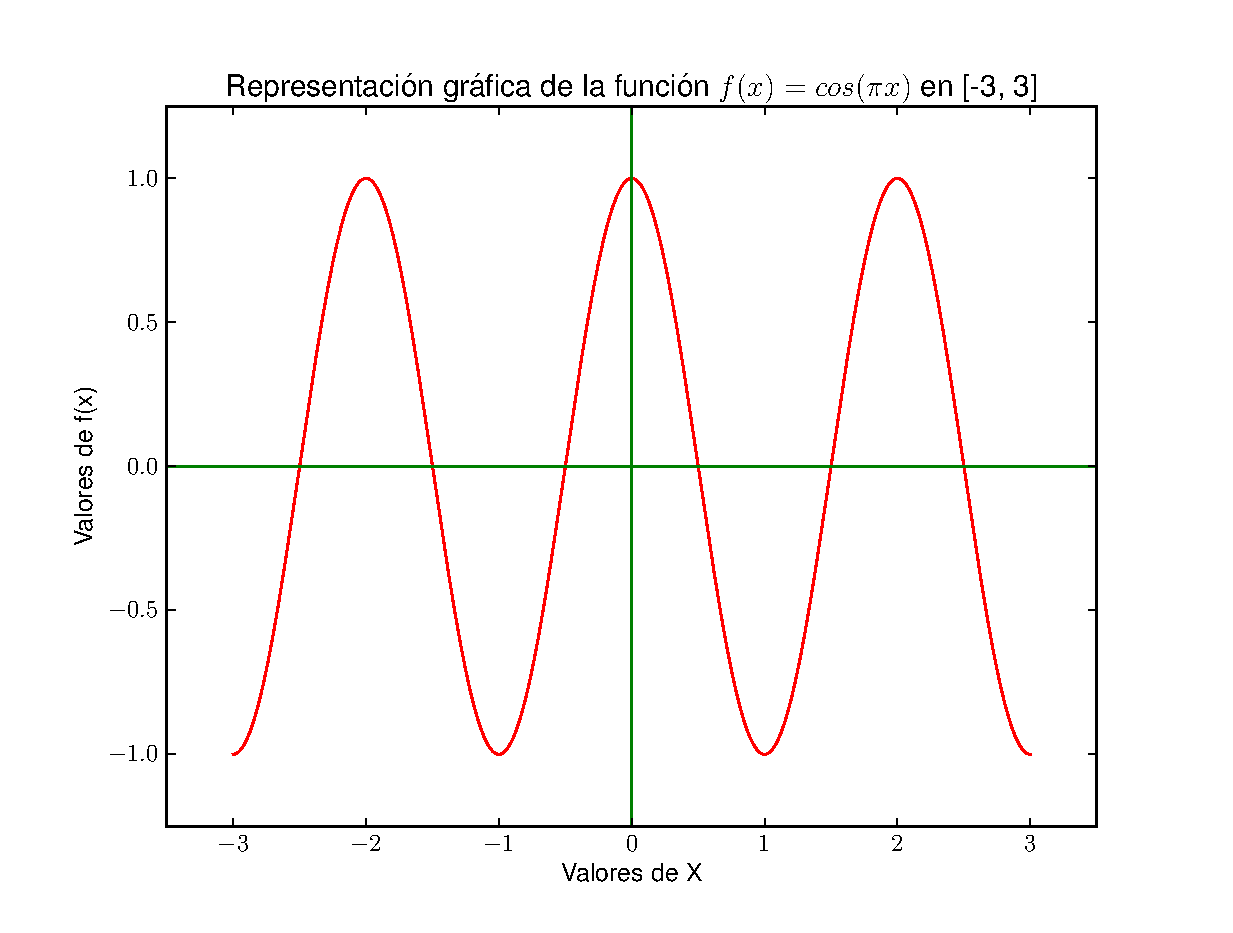
\includegraphics[height=5cm, width=6cm]{images/cos.eps}
\caption{$f(x) = cos (\pi x)$}
\label{cos}
\end{center}
\end{figure}

\end{frame}
\begin{frame}

Debido a la naturaleza del método de Newton-Raphson, es preciso señalar que su aplicación no podrá
llevarse a cabo en caso de alcanzarse una anulación de la derivada para el punto de partida del
algoritmo. Analizaremos por tanto los puntos críticos de la función de estudio, para así conocer 
qué valores deben ser evitados como suposiciones iniciales en la invocación del método:

$$(cos (\pi x))' = 0 \ \ \to \ \ -\pi sen (\pi x) = 0 $$
$$\ \ \to \ \ sen (\pi x) = 0 \ \ \to \ \ 
\pi x = k \pi, \ k \in \mathbb{Z} \ \ \to $$
$$\to \ \ x = k, \ k \in \mathbb{Z} \ \ \to x = ..., -2, -1, 1, 2, ...$$


\end{frame}
%++++++++++++++++++++++++++++++++++++++++++++++++++++++++++++++++++++++++++++++

\section{Descripción de los experimentos}

%++++++++++++++++++++++++++++++++++++++++++++++++++++++++++++++++++++++++++++++
\begin{frame}

\frametitle{Descripción de los experimentos}












  

\end{frame}
%++++++++++++++++++++++++++++++++++++++++++++++++++++++++++++++++++++++++++++++

\section{Conclusión y trabajos futuros}

%++++++++++++++++++++++++++++++++++++++++++++++++++++++++++++++++++++++++++++++
\begin{frame}
\frametitle{Conclusión y trabajos futuros}
En esta sección se facilita un resumen de las principales conclusiones alcanzadas
tras la finalización y análisis de los experimentos llevados a cabo durante la
realización del presente trabajo:

\begin{itemize}
    \item
      Las raíces de la función $f(x) = cos (\pi x)$ vienen dadas de la siguiente forma:
      $$x = \frac{1}{2} + k, \ k \in \mathbb{Z} \iff x = ..., -2.5, -1,5, -0.5, 0.5, 1.5, 2.5, ...$$
    \pause  
    \item
      Para el caso de la función de estudio, la convergencia del algoritmo de Newton-Raphson
      se encuentra prácticamente garantizada debido a la reducida separación entre raíces y 
      a su carácter de periodicidad, salvo en el caso de seleccionar un valor inicial coincidente
      con un extremo relativo de la función. 

\end{itemize} 
\end{frame}
\begin{frame}
\begin{itemize} 
    \item
      La eficiencia del algoritmo implementado resulta ser considerablemente elevada, al requerir
      ínfimos tiempos de CPU para la determinación de una raíz y no superar en ningún caso el 
      margen de cuatro iteraciones hasta obtener la solución exacta.
    \pause  
    \item
      El método de Newton-Raphson demuestra caracterizarse por una notable velocidad de convergencia
      para la función considerada, llegando a proporcionar hasta cinco cifras decimales correctas a 
      lo largo de una única iteración.
    \pause  
    \item
      Las alteraciones en los parámetros iniciales tan sólo afectan al tiempo de uso de CPU a través
      de la modificación de la cantidad total de invocaciones recursivas requeridas para alcanzar
      una raíz válida, si bien el reducido valor de dicho tiempo origina que las diferencias globales
      resulten despreciables tanto desde el punto de vista del usuario como en un sentido computacional.

\end{itemize}
\end{frame}
%++++++++++++++++++++++++++++++++++++++++++++++++++++++++++++++++++++++++++++++

\section{Bibliografía}

%++++++++++++++++++++++++++++++++++++++++++++++++++++++++++++++++++++++++++++++
\begin{frame}
  \frametitle{Bibliografía}

  \begin{thebibliography}{10}
    \beamertemplatebookbibitems
    \bibitem[Plan Estudios, 2011]{plan}
    Documento de verificación del grado.
    (2011)

    \beamertemplatebookbibitems
    \bibitem[Guía Docente, 2013]{guia}
    Guía docente.
    (2013)
    {\small $http://eguia.ull.es/matematicas/query.php?codigo=299341201$}

    \beamertemplatebookbibitems
    \bibitem[URL: CTAN]{latex}
    CTAN. {\small $http://www.ctan.org/$}


  \end{thebibliography}
\end{frame}

%++++++++++++++++++++++++++++++++++++++++++++++++++++++++++++++++++++++++++++++
\end{document}